\section{Performance}
\label{sec:result}

% original STDP paper
The discussed \ac{SNN} model has been tested using multiple different \ac{STDP} rules, as well as different training set sizes. 
Hence, there is evidence for the model's robustness and good performance in a variety of different situations, 
due to the competition among the neurons resulting in dissimilar receptive fields \cite{SNN}.
Moreover, the authors of \cite{SNN} argue that their model is more biologically plausible than other \ac{SNN} models.

However, there is a shortcoming in terms of biological fidelity of the \ac{SNN} model presented in \cite{SNN}:
Since neurons that are not in their refractory period can integrate incoming excitatory potentials and thus, 
increase their chance of firing, possibly not all neurons have the same chance of firing after the refractory period.

% STDP-like paper
The \cite{STDP_like} model was also evaluated on the MNIST dataset.
\todo{zitierung verwirrt im satzbau, es war wohl the stdb\_like model und dann erst cite gemeint}
The dataset is a suitable Benchmark for the \ac{SNN} model 
since it provides different difficulty levels of categorization.
However, the MNIST dataset is less complex than biological vision \cite{STDP_like}, 
since projections on the retina greatly vary due to object position, size, pose, illumination condition and background \cite{multi_scale_STDP}.

In addition to the accuracy with regard to the classification of the MNIST dataset impulses, \cite{STDP_like} presents \ac{RT} distributions.
\todo{hier wurde die zitierung wieder als satzbaustein verwendet}
\ac{RT} is defined as the time between the presentation of a stimulus and the response (i.e. the first pool to reach the decision threshold).
Usually, the \ac{RT} of misclassified digits is higher than the \ac{RT} of correctly classified digits.
However, the network also makes fast errors.
The results were verified with the Kolmogorov-Smirnov test, 
indicating that the correctly classified and misclassified \ac{RT} distributions are significantly different, 
whereas the distributions for stimuli from the training and test set were not \cite{STDP_like}.
\todo{nochmal}
The Kolmogorov-Smirnov test is a non-parametric test for evaluating whether two samples came from the same distribution function \cite{Kolmogorov_Smirnov}.

The performance of the \ac{SNN} model is compared for different training set sizes $n_{train}$ \cite{STDP_like}.
The results suggest that the network is able to generalize well if the training set size is sufficiently large.
The optimum training set size $n_{train} = 1000$ did not produce remarkably higher misclassification rates than bigger training set sizes \cite{STDP_like}.


% Original STDP paper
In \autoref{img:test_acc} the authors of \cite{SNN} compare the performance of the \ac{SNN} model consisting of different numbers of excitatory neurons 
and different learning rules.
The standard deviation of the test accuracy is indicated by the error bars.
The black line denotes power-law weight dependence \ac{STDP}, the red one denotes exponential weight dependence \ac{STDP}, 
the green one indicates pre-and-post \ac{STDP}, whereas the blue line's learning rule is \ac{TSTDP}.
The differences between these learning rules are explained in \cite{SNN}.
\todo{zitierung als satzbaustein}
The visualization suggests that the highest number of excitatory neurons (i.e. 6400) produces the best results for all learning rules.
The confusion matrix of \autoref{img:error_analysis} serves as an error analysis tool in \cite{SNN}.
\todo{zitierung als satzbaustein}
The authors propose possible reasons for the distribution of misclassified digits.
The most common misclassification was the digit four as a nine \cite{SNN}.

\begin{figure}[http]
    \begin{minipage}[b]{.5\linewidth}
         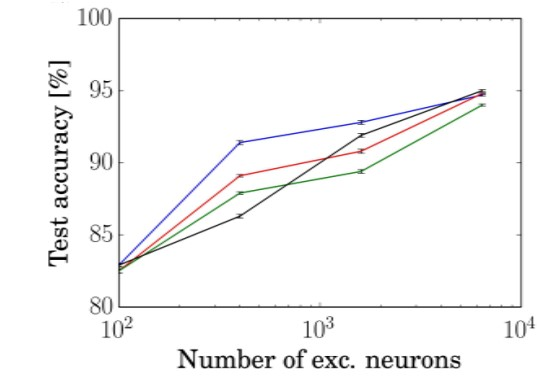
\includegraphics[width=\linewidth]{pictures/num_exc_neurons_test_acc.jpg}
         \caption{Test accuracy for different learning rules (colored lines) and different numbers of excitatory neurons from \cite{SNN}.}
         \label{img:test_acc}
    \end{minipage}
    \hspace{0.06\linewidth}% Abstand zwischen Bilder
    \begin{minipage}[b]{.4\linewidth}
         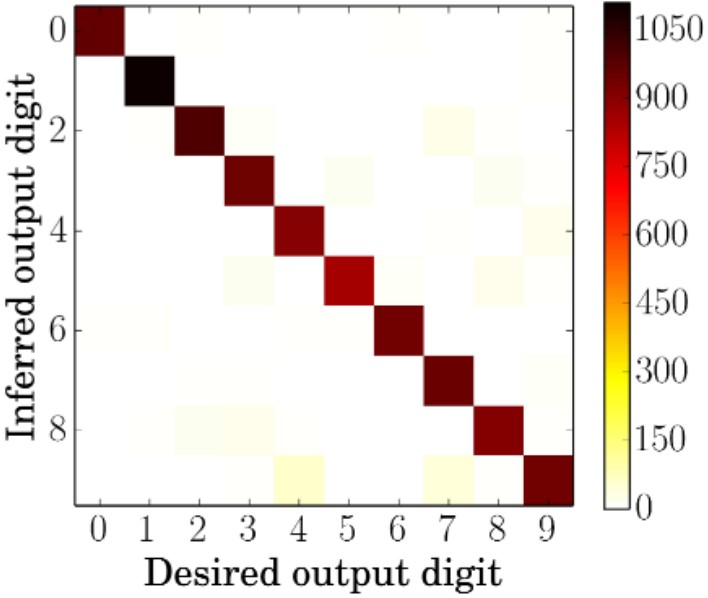
\includegraphics[width=\linewidth]{pictures/error_analysis_confusion_matrix.jpg}
         \caption{Confusion matrix presenting the average results over ten presentations of 1000 MNIST test set digits from \cite{SNN}.}
         \label{img:error_analysis}
    \end{minipage}
\end{figure}

\begin{table}[]
    \begin{tabular}{|l|l|l|l|}
    \hline
    \textbf{Training type} & \textbf{(Un-) Supervised}    & \textbf{Learning rule}               & \textbf{Performance range} \\ \hline
    Rate-based             & Supervised                   & different                            & 90-99 \%                   \\ \hline
    Spike-based            & Supervised                   & different incl. calcium variable & 91-96 \%                   \\ \hline
    Spike-based            & Unsupervised                 & rectangular/ exponential \ac{STDP}        & 93-95 \%                   \\ \hline
    \end{tabular}
    \caption{Summary of methods compared in \cite{SNN}.}
    \label{tab:different-training-types}
\end{table}
\todo{wichtig: captions von tabellen drüber, bei figures drunter}

\autoref{tab:different-training-types} is a summary of the table visualizing
performances of different \acp{SNN} in \cite{SNN}.
\todo{zitierung der tabelle passiert schon in deren caption, einmal genügt}
Rate-based learning methods achieve the best results.
Supervised methods imply the usage of a teaching signal.
%The calcium variable from the second learning rule is occasionally used to model the influence of the $Ca^{2+}$ level on activation neurons observed in biology \cite{STDP_hebbian}:
%Presynaptic action potentials release neurotransmitters that bind to certain receptors and 
%when the postsynaptic activities provide sufficient constant membrane depolarization, the $Ca^{2+}$ level rises \cite{Synaptic_plasticity}.
%A large $Ca^{2+}$ rise is associated with \ac{LTP}, whereas modest $Ca^{2+}$ rise may result in \ac{LTD} \cite{STDP_hebbian}.
The last learning rule from \autoref{tab:different-training-types} denotes the shape of the \ac{STDP} time window.